% GNUPLOT: LaTeX picture with Postscript
\begingroup
  \makeatletter
  \providecommand\color[2][]{%
    \GenericError{(gnuplot) \space\space\space\@spaces}{%
      Package color not loaded in conjunction with
      terminal option `colourtext'%
    }{See the gnuplot documentation for explanation.%
    }{Either use 'blacktext' in gnuplot or load the package
      color.sty in LaTeX.}%
    \renewcommand\color[2][]{}%
  }%
  \providecommand\includegraphics[2][]{%
    \GenericError{(gnuplot) \space\space\space\@spaces}{%
      Package graphicx or graphics not loaded%
    }{See the gnuplot documentation for explanation.%
    }{The gnuplot epslatex terminal needs graphicx.sty or graphics.sty.}%
    \renewcommand\includegraphics[2][]{}%
  }%
  \providecommand\rotatebox[2]{#2}%
  \@ifundefined{ifGPcolor}{%
    \newif\ifGPcolor
    \GPcolorfalse
  }{}%
  \@ifundefined{ifGPblacktext}{%
    \newif\ifGPblacktext
    \GPblacktexttrue
  }{}%
  % define a \g@addto@macro without @ in the name:
  \let\gplgaddtomacro\g@addto@macro
  % define empty templates for all commands taking text:
  \gdef\gplbacktext{}%
  \gdef\gplfronttext{}%
  \makeatother
  \ifGPblacktext
    % no textcolor at all
    \def\colorrgb#1{}%
    \def\colorgray#1{}%
  \else
    % gray or color?
    \ifGPcolor
      \def\colorrgb#1{\color[rgb]{#1}}%
      \def\colorgray#1{\color[gray]{#1}}%
      \expandafter\def\csname LTw\endcsname{\color{white}}%
      \expandafter\def\csname LTb\endcsname{\color{black}}%
      \expandafter\def\csname LTa\endcsname{\color{black}}%
      \expandafter\def\csname LT0\endcsname{\color[rgb]{1,0,0}}%
      \expandafter\def\csname LT1\endcsname{\color[rgb]{0,1,0}}%
      \expandafter\def\csname LT2\endcsname{\color[rgb]{0,0,1}}%
      \expandafter\def\csname LT3\endcsname{\color[rgb]{1,0,1}}%
      \expandafter\def\csname LT4\endcsname{\color[rgb]{0,1,1}}%
      \expandafter\def\csname LT5\endcsname{\color[rgb]{1,1,0}}%
      \expandafter\def\csname LT6\endcsname{\color[rgb]{0,0,0}}%
      \expandafter\def\csname LT7\endcsname{\color[rgb]{1,0.3,0}}%
      \expandafter\def\csname LT8\endcsname{\color[rgb]{0.5,0.5,0.5}}%
    \else
      % gray
      \def\colorrgb#1{\color{black}}%
      \def\colorgray#1{\color[gray]{#1}}%
      \expandafter\def\csname LTw\endcsname{\color{white}}%
      \expandafter\def\csname LTb\endcsname{\color{black}}%
      \expandafter\def\csname LTa\endcsname{\color{black}}%
      \expandafter\def\csname LT0\endcsname{\color{black}}%
      \expandafter\def\csname LT1\endcsname{\color{black}}%
      \expandafter\def\csname LT2\endcsname{\color{black}}%
      \expandafter\def\csname LT3\endcsname{\color{black}}%
      \expandafter\def\csname LT4\endcsname{\color{black}}%
      \expandafter\def\csname LT5\endcsname{\color{black}}%
      \expandafter\def\csname LT6\endcsname{\color{black}}%
      \expandafter\def\csname LT7\endcsname{\color{black}}%
      \expandafter\def\csname LT8\endcsname{\color{black}}%
    \fi
  \fi
  \setlength{\unitlength}{0.0500bp}%
  \begin{picture}(7200.00,5040.00)%
    \gplgaddtomacro\gplbacktext{%
      \csname LTb\endcsname%
      \put(990,440){\makebox(0,0)[r]{\strut{}-0.1}}%
      \put(990,922){\makebox(0,0)[r]{\strut{} 0}}%
      \put(990,1404){\makebox(0,0)[r]{\strut{} 0.1}}%
      \put(990,1885){\makebox(0,0)[r]{\strut{} 0.2}}%
      \put(990,2367){\makebox(0,0)[r]{\strut{} 0.3}}%
      \put(990,2849){\makebox(0,0)[r]{\strut{} 0.4}}%
      \put(990,3331){\makebox(0,0)[r]{\strut{} 0.5}}%
      \put(990,3812){\makebox(0,0)[r]{\strut{} 0.6}}%
      \put(990,4294){\makebox(0,0)[r]{\strut{} 0.7}}%
      \put(990,4776){\makebox(0,0)[r]{\strut{} 0.8}}%
      \put(1122,220){\makebox(0,0){\strut{} 0}}%
      \put(2559,220){\makebox(0,0){\strut{} 0.5}}%
      \put(3996,220){\makebox(0,0){\strut{} 1}}%
      \put(5433,220){\makebox(0,0){\strut{} 1.5}}%
      \put(6870,220){\makebox(0,0){\strut{} 2}}%
    }%
    \gplgaddtomacro\gplfronttext{%
      \csname LTb\endcsname%
      \put(2124,4603){\makebox(0,0)[r]{\strut{}constraints using 1:42}}%
      \csname LTb\endcsname%
      \put(2124,4383){\makebox(0,0)[r]{\strut{}constraints using 1:43}}%
      \csname LTb\endcsname%
      \put(2124,4163){\makebox(0,0)[r]{\strut{}constraints using 1:44}}%
      \csname LTb\endcsname%
      \put(2124,3943){\makebox(0,0)[r]{\strut{}constraints using 1:45}}%
      \csname LTb\endcsname%
      \put(2124,3723){\makebox(0,0)[r]{\strut{}constraints using 1:46}}%
      \csname LTb\endcsname%
      \put(2124,3503){\makebox(0,0)[r]{\strut{}constraints using 1:47}}%
      \csname LTb\endcsname%
      \put(2124,3283){\makebox(0,0)[r]{\strut{}constraints using 1:48}}%
      \csname LTb\endcsname%
      \put(2124,3063){\makebox(0,0)[r]{\strut{}constraints using 1:49}}%
      \csname LTb\endcsname%
      \put(2124,2843){\makebox(0,0)[r]{\strut{}constraints using 1:50}}%
      \csname LTb\endcsname%
      \put(2124,2623){\makebox(0,0)[r]{\strut{}constraints using 1:51}}%
      \csname LTb\endcsname%
      \put(2124,2403){\makebox(0,0)[r]{\strut{}constraints using 1:52}}%
      \csname LTb\endcsname%
      \put(2124,2183){\makebox(0,0)[r]{\strut{}constraints using 1:53}}%
      \csname LTb\endcsname%
      \put(5883,4603){\makebox(0,0)[r]{\strut{}constraints using 1:54}}%
      \csname LTb\endcsname%
      \put(5883,4383){\makebox(0,0)[r]{\strut{}constraints using 1:55}}%
      \csname LTb\endcsname%
      \put(5883,4163){\makebox(0,0)[r]{\strut{}constraints using 1:56}}%
      \csname LTb\endcsname%
      \put(5883,3943){\makebox(0,0)[r]{\strut{}constraints using 1:57}}%
      \csname LTb\endcsname%
      \put(5883,3723){\makebox(0,0)[r]{\strut{}constraints using 1:58}}%
      \csname LTb\endcsname%
      \put(5883,3503){\makebox(0,0)[r]{\strut{}constraints using 1:59}}%
      \csname LTb\endcsname%
      \put(5883,3283){\makebox(0,0)[r]{\strut{}constraints using 1:60}}%
      \csname LTb\endcsname%
      \put(5883,3063){\makebox(0,0)[r]{\strut{}constraints using 1:61}}%
      \csname LTb\endcsname%
      \put(5883,2843){\makebox(0,0)[r]{\strut{}constraints using 1:62}}%
      \csname LTb\endcsname%
      \put(5883,2623){\makebox(0,0)[r]{\strut{}constraints using 1:63}}%
      \csname LTb\endcsname%
      \put(5883,2403){\makebox(0,0)[r]{\strut{}constraints using 1:64}}%
    }%
    \gplbacktext
    \put(0,0){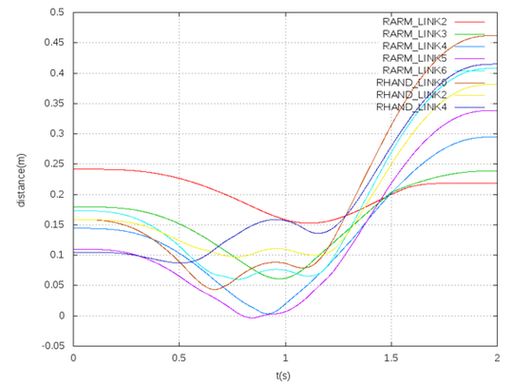
\includegraphics{distance-constraints}}%
    \gplfronttext
  \end{picture}%
\endgroup
